%; whizzy chapter -dvi
% -initex iniptex -latex platex -format platex -bibtex jbibtex -fmt fmt
% 以上 whizzytex を使用する場合の設定。

%     Tokyo Debian Meeting resources
%     Copyright (C) 2012 Junichi Uekawa
%     Copyright (C) 2011 Nobuhiro Iwamatsu

%     This program is free software; you can redistribute it and/or modify
%     it under the terms of the GNU General Public License as published by
%     the Free Software Foundation; either version 2 of the License, or
%     (at your option) any later version.

%     This program is distributed in the hope that it will be useful,
%     but WITHOUT ANY WARRANTY; without even the implied warranty of
%     MERCHANTABILITY or FITNESS FOR A PARTICULAR PURPOSE.  See the
%     GNU General Public License for more details.

%     You should have received a copy of the GNU General Public License
%     along with this program; if not, write to the Free Software
%     Foundation, Inc., 51 Franklin St, Fifth Floor, Boston, MA  02110-1301 USA

%  preview (shell-command (concat "evince " (replace-regexp-in-string "tex$" "pdf"(buffer-file-name)) "&"))
% 画像ファイルを処理するためにはebbを利用してboundingboxを作成。
%(shell-command "cd image201304; ebb *.png")

%%ここからヘッダ開始。

\documentclass[mingoth,a4paper]{jsarticle}
\usepackage{monthlyreport}

% 日付を定義する、毎月変わります。
\newcommand{\debmtgyear}{2013}
\newcommand{\debmtgmonth}{4}
\newcommand{\debmtgdate}{20}
% started from zero:
% (let ((year 2013) (month 4)) (+ (* (- year 2005) 12) month -1))
\newcommand{\debmtgnumber}{99}

\begin{document}

\begin{titlepage}
\thispagestyle{empty}
% タイトルページ:編集必要な部分は最初のマクロに飛ばすこと

\vspace*{-2cm}
第\debmtgnumber{}回 東京エリア Debian 勉強会資料\\
\hspace*{-2cm}

\includegraphics{image2012-natsu/dotdeb.pdf}\\
\hfill{}\debmtgyear{}年\debmtgmonth{}月\debmtgdate{}日

% ここはアップデートすること
% 全角文字にしないとフォントのサイズが合わないので注意
\rotatebox{10}{\fontsize{32}{32} {\gt 特集1: sambaで統合認証}}

\rotatebox{10}{\fontsize{32}{32} {\gt 特集2: 開発環境管理}}

\vspace*{-2cm}
\hfill{}
\includegraphics[height=6cm]{image200502/openlogo-nd.eps}
\end{titlepage}

\dancersection{Introduction}{上川 純一}

\begin{multicols}{2}
 

 今月のDebian勉強会へようこそ。これからDebianの世界にあしを踏み入れると
 いう方も、すでにどっぷりとつかっているという方も、月に一回Debianについ
 て語りませんか?

 Debian勉強会の目的は下記です。

 \begin{itemize}
 \item \underline{Debian Developer} (開発者)の育成。
 \item 日本語での「\underline{開発に関する情報}」を整理してまとめ、アップデートする。
 \item \underline{場}の提供。
 \begin{itemize}
  \item 普段ばらばらな場所にいる人々が face-to-face で出会える場を提供
	する。
  \item Debian のためになることを語る場を提供する。
  \item Debianについて語る場を提供する。
 \end{itemize}
 \end{itemize}		

 Debianの勉強会ということで究極的には参加者全員がDebian Packageをがりがり
 と作るスーパーハッカーになった姿を妄想しています。情報の共有・活用を通し
 て Debianの今後の能動的な展開への土台として、「場」としての空間を提供す
 るのが目的です。

\end{multicols}

\newpage

\begin{minipage}[b]{0.2\hsize}
 \definecolor{titleback}{gray}{0.9}
 \colorbox{titleback}{\rotatebox{90}{\fontsize{80}{80} {\gt デビアン勉強会} }}
\end{minipage}
\begin{minipage}[b]{0.8\hsize}
\hrule
\vspace{2mm}
\hrule
\begin{multicols}{2}
\tableofcontents
\end{multicols}
\vspace{2mm}
\hrule
\end{minipage}

\dancersection{事前課題}{上川 純一}

今回の事前課題は以下です:
\begin{enumerate}
 \item 最近Debianのアカウント・システム管理で考えていること
 \item Debianでの開発環境をどう管理しているか
\end{enumerate}
この課題に対して提出いただいた内容は以下です。
\begin{multicols}{2}
{\small
 %; whizzy-master ../debianmeetingresume201304.tex
% 以上の設定をしているため、このファイルで M-x whizzytex すると、
% whizzytexが利用できます

\begin{prework}{ べつやく }

\preworksection{最近Debianのアカウント・システム管理で考えていること}

ユーザアカウントの管理について特に意識したことがありません。ログイン時の
 パスワードを共通化できる仕組みがあるらしい・・・ぐらいの認識です。

\end{prework}

\begin{prework}{ koedoyoshida }

\preworksection{最近Debianのアカウント・システム管理で考えていること}

会社のサーバはLinux系で統一されているので、uid,gid,アカウント名をそれに合わせる程度です。
ldap連携も可能ですが、自分の管理しているマシンでは(社内向けのサービスを
 提供していないので)行っていません。

\preworksection{Debianでの開発環境をどう管理しているか}

stable環境にchrootでsid環境を作るorVMware環境上へ構築しています。

\preworksection{SambaをWindowsのドメインに参加させたことはありますか。}

「SambaをWindowsのドメインに参加させたこと」、「Linuxのユーザ認証をWindowsに統合したこと」はありません。
逆にsambaをDCとしてwindowsクライアントを参加させたことはあります。
\end{prework}

\begin{prework}{ ribbon@ns.ribbon.or.jp }

\preworksection{SambaをWindowsのドメインに参加させたことはありますか。}
あります。
\preworksection{参加させたことがある方、ハマったところを教えてください}
バージョンによって挙動が違うところです。
\end{prework}

\begin{prework}{ dictoss(杉本 典充) }

\preworksection{最近Debianのアカウント・システム管理で考えていること}

サーバで使っていても自分しか使用しないので、個人アカウントを作って完
 結してしまっている。

\preworksection{Debianでの開発環境をどう管理しているか}

amd64マシンを使っているので、i386環境はchrootで入れるように設定している。tarballを持ってきたアプリがビルド時にunameするものが一部あり、うまくビルドが通らないな場合を考えてKVM環境も併用している。ただ、ネットワーク関係のテストをするときはiptablesを使う場合が多いので最初からKVM環境で作って試している。
\end{prework}

\begin{prework}{ henrich }

\preworksection{最近Debianのアカウント・システム管理で考えていること}

Fedoraのようにユーザーがアカウントを取得して、ウェブからアクセスできる様々な活動ができるといいな、と思っています。例: https://admin.fedoraproject.org/updates

\preworksection{Debianでの開発環境をどう管理しているか}

どう管理、というのがちょっと意味が掴み取れません。普通にcowbuilderとpiupartsとlintian使ってるぐらいですが、これをどのように変更していけば効率の良い環境になるのかは知りたい所です。
\end{prework}

\begin{prework}{ 野首 }

\preworksection{最近Debianのアカウント・システム管理で考えていること}
Debianのアカウント管理は、自分の周りのマシンではいまだ/etc/passwdベース
 ばかりです。

\preworksection{Debianでの開発環境をどう管理しているか}
開発環境の管理としては、パッケージにsvn-buildpackageとgit-buildpackageを併用しています。特別使い分けたわけではなく、後になってgitを覚えてからgit-buildpackageを使ってみただけなので、これに特別な利点があったりはしません。むしろ設計思想が全然違うので一本化できず困っています。
あとはsid環境にlxcを使ってみたり、armやsparcのテストのためにqemuを使い始めたりしている程度です。

\end{prework}

\begin{prework}{ 石井一夫 }

\preworksection{最近Debianのアカウント・システム管理で考えていること}

セキュリティは結構深刻で、内部の者も悪さをする恐れがあり、かなり、気を使います。サーバでは、一般ユーザにsudo権限を取得できないようにし、管理者用アカウントを作ってwheel のグループに所属させ、それだけが、sudo権限を取得できるようにしています。パスワードは、3ヶ月ごとに変更。Kerberosは気になりますが、使いこなせていません。

\preworksection{Debianでの開発環境をどう管理しているか}

GCCとか、JDKとかインストールできるものは、可能な限りインストールしていますが、環境管理とまでは行っていません。これからの課題です。
\end{prework}

\begin{prework}{ 上川純一 }

\preworksection{最近Debianのアカウント・システム管理で考えていること}

個人の環境は自分と目的用途別に作っているアカウントで、自分のアカウント以
外はインタラクティブに利用する用途ではないので基本的にはパスワードを設
定せず利用しています。

昔はファイル共有でNFSを使っていたのでシステム間でUIDを一致させないといけないなどの面
倒がありましたが最近はsshfs とか rsync/ssh でファイルを共有するので片方向
の鍵認証でファイルのアクセス権が決まるモデルになっています。こっちのほう
が管理者としてはやりやすいですね。

\preworksection{Debianでの開発環境をどう管理しているか}

cowbuilderでamd64 sidの環境のみを維持管理しています。昔はいろいろなCPUアー
 キテクチャーとかOSをとかをためしていたので大量のイメージがありました。
cowbuilder だと常に最新版のバイナリを使うことになります。また、必要なソ
 フトウェアを必要なときにJust In Timeでインストールしてくれることになり
 ます。
OSイメージの構成・履歴管理などを省略してくれるのでいいです。

開発環境の仮想マシンを管理するとどういうメモリを割り当てるかとかネットワー
クの設定をどうするかだとかというのも心配することになるんですが、
cowbuilderではホストOSの環境をそのままつかっているので楽です。開発環境の
メンテナンスが目的ではなく開発環境を使うことが目的なので開発環境はメンテ
ナンスフリーなのが理想だと思います。

各種クラウドサービスを使うとOSイメージのインストールからさせられることが
多いのですがそこではじめていかに世間の人が環境の維持管理を重要なタスクだ
と思っていて、cowbuilderが楽なのかを認識した気がします。

\end{prework}

\begin{prework}{ まえだこうへい }

\preworksection{最近Debianのアカウント・システム管理で考えていること}

Debianの、というかLDAPに代わるもっとシンプルなアカウント管理の仕組みを作りたいなと思っているだけで何もやってません。

\preworksection{Debianでの開発環境をどう管理しているか}

Pythonでのツールの開発はのSidを使っていますが、Sid自体はVirtual Box上にあるので、Shutdown時に都度snapshotを取っています。

\preworksection{SambaをWindowsのドメインに参加させたことはありますか。}

某所でSamba使っていましたが、某所のADには参加できない(その某所とは別の法人組織だったので)が、アクセスは某所のPCでしかできないので、ユーザアカウントを同一にするため、某所のシステムからユーザアカウント引っこ抜いてLDIFに変換してLDAPでアカウント管理してました。(Sambaとは直接連携してない)
\end{prework}

\begin{prework}{ 吉野(yy\_{}y\_{}ja\_{}jp) }

\preworksection{最近Debianのアカウント・システム管理で考えていること}

スタンドアロンで使うとき,VMで使うときがありますがどちらも考える必要を感じてません.

\preworksection{Debianでの開発環境をどう管理しているか}

どちらの場合も特に何もしてないです.

\preworksection{SambaをWindowsのドメインに参加させたことはありますか。}
ありません.
\preworksection{Linuxのユーザ認証をWindowsに統合したことはありますか。}
ありません.

\end{prework}

\begin{prework}{ 岩松 信洋 }

\preworksection{最近Debianのアカウント・システム管理で考えていること}

特にアカウント管理に関して考えてないです。
昔ながらのユーザとグループで管理しています。

\preworksection{Debianでの開発環境をどう管理しているか}

chroot と alias, シェルスクリプトによる切り替えを使っています。

\preworksection{「SambaをWindowsのドメインに参加させたことはありますか。参加させたことがない方、もしお時間があれば実際にやってみて、ハマったところを教えてください。参加させたことがある方、ハマったところを教えてください。」、「Linuxのユーザ認証をWindowsに統合したことはありますか。ある場合はその際の方法やハマったところについて教えてください。ない場合は、もしお時間があれば実際にやってみてハマったところを教えてください」にお答えください。}

誰でもアクセスできるようなsambaサーバしか構築したことないので、特にハマったということはないです。
\end{prework}

}
\end{multicols}

\dancersection{Debian Trivia Quiz}{上川純一}

ところで、みなさん Debian 関連の話題においついていますか?Debian関連の話
題はメーリングリストをよんでいると追跡できます。ただよんでいるだけではは
りあいがないので、理解度のテストをします。特に一人だけでは意味がわからな
いところもあるかも知れません。みんなで一緒に読んでみましょう。

今回の出題範囲は\url{debian-devel-announce@lists.debian.org} や \url{debian-devel@lists.debian.org}に投稿された
内容とDebian Project Newsからです。

\begin{multicols}{2}
 %; whizzy-master ../debianmeetingresume201304.tex
% 以上の設定をしているため、このファイルで M-x whizzytex すると、whizzytexが利用できます。
%

\santaku
{DSAのサーバを新しくホスティングしてくれるのはどれか}
{bytemark}
{grnet}
{manda}
{A}
{Debianプロジェクトのサーバ管理を担うチームがDSA、
その管理するDebianサーバのホスティングは、grnet, manda, ubcece が既存のホスティングプロバイダーで、bytemarkが今回
加わったそうです。}

\santaku
{wheezy の backports の apt-lineで適切なものはどれか}
{deb sstp://backports.debian.org/debian/ wheezy-backports backports}
{deb http://backports.debian.org/debian/ wheezy-backports main}
{deb http://ftp.debian.org/debian/ wheezy-backports main}
{C}
{backports がメインのアーカイブと統合されたようで、wheezy-backportsから
利用できるようになったようです。}

\santaku
{tech ctte 699808の結果アップロードされたのは}
{syslinux 4}
{syslinux 5}
{grub}
{A}
{新しいバージョンのsyslinuxでdebian-installerが動かないという問題があっ
てそれをダウングレードで解決したようです。}

\santaku
{あたらしくDPLになったのはだれか}
{Stephano Zacchiroli}
{Lucas Nussbaum}
{Gergely Nagy}
{B}
{Lucas が選挙の結果DPLになりました}

% \santaku
% {}
% {}
% {}
% {}
% {}
% {}


% \santaku
% {}
% {}
% {}
% {}
% {}
% {}

\end{multicols}

%-------------------------------------------------------------------------------
\dancersection{Debian勉強会予約システム変更履歴}{上川純一}
%-------------------------------------------------------------------------------
\index{Debianべんきょうかいよやくしすてむ@Debian勉強会予約システム}

Debian勉強会の予約システムの機能をいくつか変更したので報告します。

\subsection{アンケートのリマインダ}

\begin{wrapfigure}{r}{30zw}
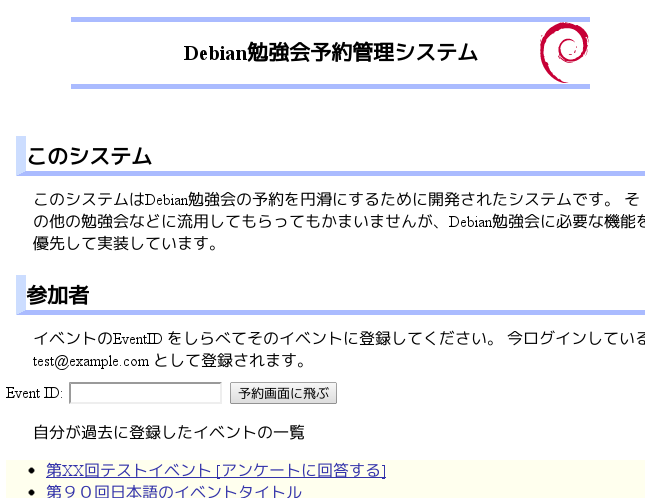
\includegraphics[width=1\hsize]{image201304/enquetereminder.png}
\end{wrapfigure}

アンケートを送付していますが、現状メールで通知しているのみで、メールから
しかアンケート回答できません。
勉強会に登録している場合にアンケートを依頼してもメールがとどいていないと
かメールに気づいていないというフィードバックをもらいました。

しかしながらメール通知以外で勉強会のあとにウェブページに来てもらうという
のは難しいと思うのですが、ものは試しという事でトップページにリンクを表示
するようにして見ました。参加しているイベントでアンケートの質問が作成され
ていてアンケートの回答がまだなされていない場合にアンケートのリンクを表示
します。


\subsection{勉強会に登録した時刻}

SVGでなにができるのか試してみる勉強のついでに勉強会幹事用のページにグラ
フを出すようにして見ました。時刻を10に分割してそれぞれの時刻においての
登録の頻度の推移をみれるようにしています。このグラフを見ることでどのイベ
ントでいつごろ何人登録したのかがわかります。
試しに最近の二回を見てみたのですがけっこう違いますね。

HTML5 においてSVGの画像をうめこむのは結構簡単で、そのままSVGタグを埋め込め
ばいいだけです。inkscapeの吐くSVGをみて手書きは無理かなと思っていたので
すが基本的な記法だけであれば手書きするのも悪くはないと思える書式でした。
\index{svg}

\begin{commandline}
 <svg width="800" height="120">
	  <text x="0" y="120">2012-11-03</text>
	  <text x="400" y="120">2012-11-17</text>
	  <text x="0" y="100">0</text>
	  <text x="0" y="16">6</text>
	  <polyline points="
 0,83.3333333333
 50,66.6666666667
 100,83.3333333333
 150,100.0
 200,100.0 
 250,100.0 
 300,100.0 
 350,100.0 
 400,0.0 
 450,33.3333333333 " 
          fill="none" stroke="#333">
	  </polyline>
    </svg>
\end{commandline}

\begin{figure}[ht]
\begin{minipage}{0.5\hsize}
 \begin{center}
  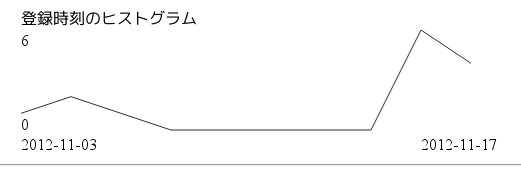
\includegraphics[width=1\hsize]{image201304/attendgraph1.png}
 \end{center} 
 \caption{2012年11月の勉強会の登録時刻}
\end{minipage}
\begin{minipage}{0.5\hsize}
\begin{center}
  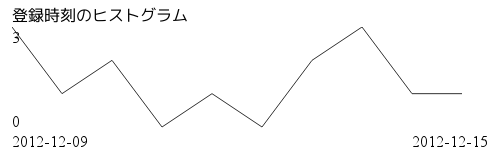
\includegraphics[width=1\hsize]{image201304/attendgraph2.png}
\end{center} 
\caption{2012年12月の勉強会の登録時刻}
\end{minipage}
\end{figure}

\subsection{コミット数}

\begin{wrapfigure}{r}{30zw}
\begin{center}
\includegraphics[width=1\hsize]{image201304/util-gae-commits.eps}
\end{center}
\caption{各四半期毎におけるutil/gaeディレクトリのgitコミット数}
\end{wrapfigure}

気になったのでコミット数のグラフを作成してみました。四半期ごとにプロット
しています。年末に集中してコミットしているのが見て取れます。しばらくいじっ
てない気がしていましたが年に一回くらいは頑張っていじってる時期があるみた
いですね。一年を振り返るついでにいろいろ弄りたくなるのかもしれません。


%-------------------------------------------------------------------------------
\dancersection{debootstrapを有効活用してみよう}{杉本典充}
%-------------------------------------------------------------------------------
\index{debootstrap}

debianのインストール処理に使うdebootstrapコマンドの応用例として開発環境整備、サーバ用途、組み込み用途、異種OS利用とまとめてみました。

\subsection{仮想化技術について}
最近KVMを事例とする「仮想化」という言葉をよく聞くようになりました。仮想化にもいくつかの種類があると思い調べてみたところ、以下の例が見つかりました。今回は、コンテナ型仮想化に着目していきます。

\begin{table}[hb]
  \begin{tabular}{|l|p{10em}|p{20em}|} \hline
    仮想化技術 & 実装例 & 仮想化環境の特徴 \\ \hline
    完全仮想化(エミュレーション型) & QEMU、VirtualBox & 既存のOSを無修正のままゲスト環境として動作させる。ホストOSで動作する仮想化アプリケーションがエミューションする。 \\ \hline
    完全仮想化(ハイパーバイザ型) & KVM & 既存のOSを無修正のままゲスト環境として動作させる。CPU等の仮想化機能を使うことでホスト環境におけるオーバーヘッドを極力減らしている。 \\ \hline
    準仮想化 & Xen & ホスト環境とやりとりするAPIを利用できるように修正が入ったOSをゲストOSとして動作させる方式(=既存のOSそのままでは動かない) \\ \hline
    コンテナ型仮想化 & OpenVZ、LXC、FreeBSD jail & ホスト環境とゲスト環境は同一カーネルで動作しつつ、ホスト環境から分離したゲスト環境を提供する。  \\ \hline
  \end{tabular}
\end{table}

\subsection{debianにおけるコンテナ環境の作り方}

\subsubsection{debootstrap}
debianにおいてコンテナ型仮想化の環境を構築する機能としてdebootstrapがあります。debootstrapを実行すると、debianをインストールしたときのルートディレクトリ構造を任意のパスに作成することができます。

debootstrapのインストールは以下のapt-getコマンドで実行できます。deboostrapにはdebootstrap(shスクリプトで実装)とcdebootsrap(C言語で実装)の2種類のコマンドがあります。

\begin{commandline}
$ sudo apt-get install debootstrap cdebootstrap
$ sudo mkdir -p /srv/chroot
$ cd /srv/chroot
$ sudo debootstrap --arch=amd64 sid ./mysid http://ftp.jp.debian.org/debian
$ ls mysid
bin   dev  home  lib64  mnt  proc  run   selinux  sys  usr
boot  etc  lib   media  opt  root  sbin  srv      tmp  var
\end{commandline}

\subsubsection{chrootコマンド}
debootstrapで作成したコンテナ環境でプログラムを実行したいのですが、環境変数とディレクトリの配置が合わないためうまくコマンドを実行することができません。そこでchrootコマンドを使います。\footnote{chrootシステムコールは1982年にビル・ジョイが作成したものが起源とされています。ビル・ジョイはプログラムをクリーンビルドできる環境がほしかったため通常利用の環境と分離する手段として開発したと言われています。} \footnote{クリーンビルド目的でchrootコマンドを使う手法ではdebianパッケージのビルドにも使われています。}

chrootコマンドを実行するとルートディレクトリでない場所をあたかもルートディレクトリであるように見せることができます。これにより普通にdebianをインストールした状態のプログラムの配置とPATH環境変数がうまく合い、コンテナ環境のプログラムを実行できるようになります。

\begin{commandline}
$ sudo chroot /srv/chroot/mysid
# pwd
/
# ls
bin   dev  home  lib64  mnt  proc  run   selinux  sys  usr
boot  etc  lib   media  opt  root  sbin  srv      tmp  var
\end{commandline}

chrootコマンドにも現在ではいくつかの派生版があります。

\begin{itemize}
  \item chroot
  \begin{itemize}
    \item 元祖chroot。実行するにはroot権限が必要。
  \end{itemize}
  \item dchroot
  \begin{itemize}
    \item chrootを一般ユーザで実行できるように改良した版。(とはいえdebootstrapと設定ファイル作成はroot権限が必要)
  \end{itemize}
  \item schroot
  \begin{itemize}
    \item dchrootのセキュリティレベルを向上させた改良版。
  \end{itemize}
\end{itemize}

今度はschrootコマンドでコンテナ環境に入ってみます。

\begin{commandline}
$ sudo apt-get install schroot
$ cd /etc/schroot
$ sudo vi schroot.conf

[mysid]
description=my sid for devel
type=directory
directory=/srv/chroot/mysid
users=norimitu
root-groups=root
personality=linux
preserve-environment=true

$ schroot -c mysid
W: Failed to change to directory ‘/etc/schroot’: No such file or directory
I: The directory does not exist inside the chroot.  Use the --directory option to run the command in a different directory.
W: Falling back to directory ‘/home/norimitu
$ ls -la /srv
total 8
drwxr-xr-x  2 root root 4096 Apr 14 02:59 .
drwxr-xr-x 22 root root 4096 Apr 14 03:04 ..

(何もないです。chroot環境に入っています)
$ cd /home/norimitu
$ ls
(chroot元のホスト環境のファイルが出てくる。)
\end{commandline}

直感的にはchrootコマンドの方がわかりやすいです。

schrootコマンドの場合は、schrootした環境内のホームディレクトリはホスト環境のホームディレクトリとbindされます。そのため、ホスト環境にあるファイルをschrootした環境からそのまま読み書きできます。(chrootの場合はそういう仕組みがないため、コピーする必要がある。)

\subsection{debootstrapの使いどころ}

debootstrapを使うと何が便利なのか使いどころの例を上げてみます。

\subsubsection{生活環境と開発(テスト)環境を分離する}

普段使用する環境はstableを利用するが、バージョン等の都合で部分的にsidで提供されているパッケージを利用したい場合があります。その場合、前述した方法でコンテナ環境を作成し、chrootすれば利用できます。

\subsubsection{コンテナ内で異なるCPUアーキテクチャの環境を動かす}

debootstrapしたコンテナ環境は通常ホスト環境で動作するCPUアーキテクチャで構築します。chrootコマンドでコンテナ環境に入っている場合でもカーネルはホストOSと同じため、異なるCPUアーキテクチャのバイナリをネイティブに実行できないためです。

amd64カーネルを実行しているマシンの場合、i386バイナリは実行できますのでi386環境のコンテナ環境を構築すれば実行できます。

私は諸般の都合でi386のpostgresql-9.1を動かしてVPSへレプリケーションしていますが、amd64とi386間といったCPUアーキテクチャが異なる場合にレプリケーションができない仕様となっているため、VPSのホストOSはamd64、コンテナ内でi386環境を動かしてレプリケーションしています。

% personality flags も考えると多分 linux32 コマンド使ったほうが良いと思
% う --dancerj
\begin{commandline}
$ sudo mkdir -p /srv/chroot
$ cd /srv/chroot
$ sudo debootstrap --arch=i386 sid ./mysid-i386 http://ftp.jp.debian.org/debian
$ sudo chroot ./mysid-i386
# uname -a
Linux www6368uj 3.2.0-4-amd64 #1 SMP Debian 3.2.41-2 x86_64 GNU/Linux
# apt-get install file
# file /bin/ls
/bin/ls: ELF 32-bit LSB executable, Intel 80386, version 1 (SYSV),
dynamically linked (uses shared libs), for GNU/Linux 2.6.26,
BuildID[sha1]=0x498625fc854816515ec12819544ebedff51d5c32, stripped
\end{commandline}

 また、chrootとQEMUを組み合わせることにより、ホストOSのカーネルでは動作しないCPUアーキテクチャのコンテナ環境をQEMUを使ったエミュレートで動作させることができます。最近流行りの安価なARMボードでdebianを動作させるためのディレクトリツリーを作成するのに便利です。\footnote{実際にARMボード上でdebianを起動させるためにはSDカード等へのファイルシステム作成、カーネルやドライバの作成、ブートローダーの書き込み等、色々やらないと動きません。}

 ホスト環境と異なるCPUアーキテクチャのコンテナ環境をchrootする場合、以下の手順で実行する必要があります。

\begin{itemize}
  \item debootstrapは「--foreign」引数を渡して実行すること
  \item コンテナ環境内に「qemu-*-static」ファイルをコピーしておくこと(例:qemu-arm-static)
  \item chrootで入った後でdebootstrapのsecond stageを実行すること
\end{itemize}

\begin{commandline}
$ sudo apt-get install binfmt-support qemu qemu-user-static debootstrap
$ sudo mkdir -p /srv/chroot
$ cd /srv/chroot
$ sudo debootstrap --foreign --arch=armel wheezy ./armdev1 http://ftp.jp.debian.org/debian
$ sudo chroot ./armdev1
chroot: コマンド `/bin/bash' の実行に失敗しました: No such file or directory

$ sudo cp /usr/bin/qemu-arm-static /srv/chroot/armdev1/usr/bin/
$ sudo chroot armdev1
I have no name!@hostname:/#
Linux hostname 3.2.0-4-amd64 #1 SMP Debian 3.2.41-2 armv7l GNU/Linux

I have no name!@hostname:/# apt-get update
bash: apt-get: command not found
I have no name!@hostname:/# ls /debootstrap
arch  debootstrap      debpaths        functions  suite
base  debootstrap.log  devices.tar.gz  required   suite-script
I have no name!@hostname:/# /debootstrap/debootstrap --second-stage
I: Installing core packages...
I have no name!@hostname:/# apt-get update
Reading package lists...

I have no name!@hostname:/# vi /etc/apt/sources.list

deb http://ftp.jp.debian.org/debian wheezy main
deb-src http://ftp.jp.debian.org/debian wheezy main

deb http://security.debian.org/ wheezy/updates main
deb-src http://security.debian.org/ wheezy/updates main

I have no name!@hostname:/# apt-get update
I have no name!@hostname:/# apt-get install file
I have no name!@hostname:/# file /bin/ls
/bin/ls: ELF 32-bit LSB executable, ARM, version 1 (SYSV),
dynamically linked (uses shared libs), for GNU/Linux 2.6.26,
BuildID[sha1]=0x5bc97dbca9ac168932d898a5e2eaf68e8fde5e16, stripped
\end{commandline}


\subsubsection{サーバでたくさんのコンテナを常駐させて動かしたい}

今までのコンテナ環境は手でコマンドを実行することでコンテナ環境に入っていました。コンテナ環境をサーバのように動かしたいというニーズもあります。今回はDebian GNU/Linux wheezy amd64上でLXC(Linux Containers)を用いてコンテナ環境を常駐させてみます。

まずホスト環境の設定と環境を確認します。

\begin{commandline}
$ sudo apt-get install lxc
$ sudo vi /etc/fstab

(追記します)
cgroup  /sys/fs/cgroup  cgroup  defaults  0   0

$ sudo mount -a
$ lxc-checkconfig
Kernel config /proc/config.gz not found, looking in other places...
Found kernel config file /boot/config-3.2.0-4-amd64
--- Namespaces ---
Namespaces: enabled
Utsname namespace: enabled
Ipc namespace: enabled
Pid namespace: enabled
User namespace: enabled
Network namespace: enabled
Multiple /dev/pts instances: enabled

--- Control groups ---
Cgroup: enabled
Cgroup clone_children flag: enabled
Cgroup device: enabled
Cgroup sched: enabled
Cgroup cpu account: enabled
Cgroup memory controller: enabled
Cgroup cpuset: enabled

--- Misc ---
Veth pair device: enabled
Macvlan: enabled
Vlan: enabled
File capabilities: enabled

Note : Before booting a new kernel, you can check its configuration
usage : CONFIG=/path/to/config /usr/bin/lxc-checkconfig
\end{commandline}

LXCで動作するコンテナ環境のネットワークはホスト環境とブリッジ接続する必要があります。

ここではeth0はそのままでブリッジデバイスを1つ作成し、LXCのコンテナ環境はブリッジデバイスのNAT環境下で動作することとします。\footnote{http://wiki.debian.org/LXC/SimpleBridge}

\begin{commandline}
$ sudo vi /etc/sysctl.conf

(変更)
net.ipv4.ip_forward=1

$ sudo sysctl -p
net.ipv4.ip_forward = 1

$ vi br-lxc.sh
# script to setup a natted network for lxc guests
CMD_BRCTL=/sbin/brctl
CMD_IFCONFIG=/sbin/ifconfig
CMD_IPTABLES=/sbin/iptables
CMD_ROUTE=/sbin/route
NETWORK_BRIDGE_DEVICE_NAT=lxc-bridge-nat
HOST_NETDEVICE=eth0
PRIVATE_GW_NAT=192.168.20.1
PRIVATE_NETMASK=255.255.255.0
PRIVATE_NETWORK=192.168.20.0/24

${CMD_BRCTL} addbr ${NETWORK_BRIDGE_DEVICE_NAT}
${CMD_BRCTL} setfd ${NETWORK_BRIDGE_DEVICE_NAT} 0

${CMD_IFCONFIG} ${NETWORK_BRIDGE_DEVICE_NAT} ${PRIVATE_GW_NAT} netmask ${PRIVATE_NETMASK} promisc up

${CMD_IPTABLES} -t nat -A POSTROUTING -o ${HOST_NETDEVICE}  -j MASQUERADE
${CMD_IPTABLES} -A FORWARD -i ${NETWORK_BRIDGE_DEVICE_NAT} -o ${HOST_NETDEVICE} -s ${PRIVATE_NETWORK} -j ACCEPT

$ sudo ./br-lxc.sh
$ sudo ifconfig lxc-bridge-nat
lxc-bridge-nat Link encap:イーサネット  ハードウェアアドレス fe:24:c3:eb:6d:c3
          inetアドレス:192.168.20.1 ブロードキャスト:192.168.20.255  マスク:255.255.255.0
          inet6アドレス: fe80::409a:3cff:fee6:33b0/64 範囲:リンク
          UP BROADCAST RUNNING PROMISC MULTICAST  MTU:1500  メトリック:1
          RXパケット:6556 エラー:0 損失:0 オーバラン:0 フレーム:0
          TXパケット:1121 エラー:0 損失:0 オーバラン:0 キャリア:0
      衝突(Collisions):0 TXキュー長:0
          RXバイト:543131 (530.4 KiB)  TXバイト:95778 (93.5 KiB)
\end{commandline}

コンテナを作成します。LXCにおけるコンテナは ``\texttt{/var/lib/lxc}''ディレクトリの下にできます。

\begin{commandline}
$ sudo lxc-create -n lxc-deb1 -t debian
 (ダイアログ形式でインストールするバージョンやダウンロード先ミラーのURL、
  rootパスワードが聞かれるので答える) 

$ cd /var/lib/lxc/lxc-deb1
$ ls
config    rootfs
$ sudo vi config

(追記します)
## Network
lxc.utsname = lxc-deb1
lxc.network.type = veth
lxc.network.flags = up

# that's the interface defined above in host's interfaces file
lxc.network.link = lxc-bridge-nat

# name of network device inside the container,
# defaults to eth0, you could choose a name freely
# lxc.network.name = lxcnet0

lxc.network.hwaddr = 00:FF:AA:00:00:01

# the ip may be set to 0.0.0.0/24 or skip this line
# if you like to use a dhcp client inside the container
lxc.network.ipv4 = 192.168.20.101/24
\end{commandline}

LXCコンテナ内でsshdが起動するよう設定しておきます。

\begin{commandline}
$ sudo cp /etc/resolv.conf /var/lib/lxc/lxc-deb1/rootfs/etc/
$ sudo vi /var/lib/lxc/lxc-deb1/rootfs/etc/ssh/sshd_config

(変更前)  #ListenAddress 0.0.0.0
(変更後)  ListenAddress 192.168.20.101 
\end{commandline}

LXCコンテナを起動します。``-d''オプションはバックグラウンドで起動させるオプションです。これでコンテナ環境が常駐して動作するようになります。

\begin{commandline}
$ sudo lxc-start -n lxc-deb1
Using makefile-style concurrent boot in runlevel 2.
Starting OpenBSD Secure Shell server: sshdCould not load host key: /etc/ssh/ssh_host_rsa_key
Could not load host key: /etc/ssh/ssh_host_dsa_key

なぜかssh鍵を作る処理が自動実行されず止まってしまうため、手動で作ってみる。
$ sudo chroot /var/lib/lxc/lxc-deb1/rootfs ssh-keygen -t dsa -f /etc/ssh/ssh_host_dsa_key
$ sudo chroot /var/lib/lxc/lxc-deb1/rootfs ssh-keygen -t rsa -f /etc/ssh/ssh_host_rsa_key

$ sudo lxc-start -n lxc-deb1 -d
$ ssh root@192.168.20.101
root@lxc-deb1:~#

 ログインできました。

$ sudo lxc-stop -n lxc-deb1
\end{commandline}

\subsubsection{異なるOS上でdebianを構築する}

debootstrapは異なるOS上でdebianを構築することができます。ここでは、FreeBSD-8.3-RELEASE amd64のjail機能を用いてkfreebsd-amd64をprisonerとして動かしてみます。\footnote{http://blog.vx.sk/archives/22-Updated-Tutorial-Debian-GNUkFreeBSD-in-a-FreeBSD-jail.html}

まずはjail環境を作成するためのツールをインストールします。

OSが異なるとdebootstrapコマンドがないため、tarball(中身はshスクリプト版)をダウンロードして実行します。\footnote{portsで/usr/ports/sysutils/debootstrapもありますのでそちらを使ってもいいです}

\begin{commandline}
> cd
> wget http://ftp.jp.debian.org/debian/pool/main/d/debootstrap/debootstrap_1.0.48.tar.gz
> tar xf debootstrap_1.0.48.tar.gz
> cd debootstrap-1.0.48
# su
# setenv DEBOOTSTRAP_DIR `pwd`
# ./debootstrap --arch=kfreebsd-amd64 wheezy /usr/jails/jailkfdeb http://ftp.jp.debian.org/debian
# kldload fdescfs linprocfs linsysfs tmpfs
# umount /usr/jails/jailkfdeb/dev/fd
# umount /usr/jails/jailkfdeb/dev
# mount -t linprocfs linprocfs /usr/jails/jailkfdeb/proc
# mount -t linsysfs linsysfs /usr/jails/jailkfdeb/sys
# mkdir -p /usr/jails/jailkfdeb/lib/init/rw
# mount -t tmpfs tmpfs /usr/jails/jailkfdeb/lib/init/rw
# cp /etc/resolv.conf /usr/jails/jailkfdeb/etc/resolv.conf
\end{commandline}

\begin{commandline}
> sudo portsnap fetch
> sudo portsnap update
> cd /usr/ports/sysutils/ezjail
> sudo make
> sudo make install

> sudo touch /etc/fstab.jailkfdeb
  (このファイルがないとエラーになるためとりあえず作成します)
> vi /etc/rc.conf
(追記します)
ifconfig_em0_alias0="inet 192.168.1.63/32"

> ifconfig em0 192.168.1.63 netmask 255.255.255.255 alias
> vi /usr/local/etc/ezjail/jailkfdeb

# To specify the start up order of your ezjails, use these lines to
# create a Jail dependency tree. See rcorder(8) for more details.
#
# PROVIDE: standard_ezjail
# REQUIRE:
# BEFORE:
#

export jail_jailkfdeb_hostname="jailkfdeb"
export jail_jailkfdeb_ip="192.168.1.63"
export jail_jailkfdeb_rootdir="/usr/jails/jailkfdeb"
export jail_jailkfdeb_exec_start="/etc/init.d/rc 3"
export jail_jailkfdeb_exec_stop=""
export jail_jailkfdeb_flags="-l -u root"
export jail_jailkfdeb_mount_enable="YES"
export jail_jailkfdeb_devfs_enable="YES"
export jail_jailkfdeb_devfs_ruleset="devfsrules_jail"
export jail_jailkfdeb_procfs_enable="YES"
export jail_jailkfdeb_fdescfs_enable="YES"


> sudo /usr/local/etc/rc.d/ezjail start jailkfdeb
Configuring jails:.
Starting jails: jailkfdeb.
> jls
   JID  IP Address      Hostname                      Path
    11  192.168.1.63    jailkfdeb                     /usr/jails/jailkfdeb
> jexec 11 /bin/sh

(ここからコンテナ環境の中です)

# uname -irps
GNU/kFreeBSD 8.3-RELEASE-p6 amd64 Intel(R) Core(TM) i5-2500S CPU @ 2.70GHz
# vi /etc/apt/sources.list

deb http://ftp.jp.debian.org/debian wheezy main contrib non-free
deb-src http://ftp.jp.debian.org/debian wheezy main contrib non-free

# apt-get update
# apt-get install openssh-server
# vi /etc/ssh/sshd_config

修正前)  #ListenAddress 0.0.0.0
修正後)  ListenAddress 192.168.1.63

# /etc/init.d/ssh restart
# passwd
# exit

(コンテナ環境からホスト環境に戻ります)

> ssh root@192.168.1.63 
\end{commandline}

sshでコンテナ環境にログインできました。

\subsection{参考情報}

\begin{itemize}
  \item{Debian Wiki Schroot http://wiki.debian.org/Schroot}
  \item{Debian Wiki LXC http://wiki.debian.org/LXC}
  \item{Debian Wiki EmDebianCrossDebootstrap http://wiki.debian.org/EmDebian/CrossDebootstrap}
  \item{関西エリアDebian勉強会 2009年04月号「Debian を新規に install してから常用環境にするまで」 佐々木洋平}
  \item{Updated Tutorial: Debian GNU/kFreeBSD in a FreeBSD jail  http://blog.vx.sk/archives/22-Updated-Tutorial-Debian-GNUkFreeBSD-in-a-FreeBSD-jail.html}
\end{itemize}

\dancersection{Samba で Linux の認証を Windows に統合してみたり}{たかはしもとのぶ}
\index{samba}

\subsection{無慈悲な一言、言われませんかw}
Windowsの大群の中でLinuxサーバを運用しているとよく言われるのが、「その(Linux)サーバの認証、Active Directoryでできないの?」という大変無慈悲な(笑)一言ではないでしょうか。ということで、今回はSambaを使ってLinuxサーバの認証をWindowsに統合する方法について、いろいろご紹介していきたいと思います。
\index{active directory}

\subsection{Sambaって$\cdots \cdots$}
一応説明しておきますと、Debianを含むUNIX系 OS 上でファイル共有をはじめとするWindowsサーバの各種機能を実現するオープンソースのソフトウェアです。元々はファイル共有、プリンタ共有の機能から出発していますが、最近ではWindowsの中核機能であるActive Directoryのドメインコントローラ機能や、Windowsドメインのクライアント機能など、多くの機能を実装しています。

ただ、そのあたりの機能の紹介をしていると、SambaというよりWindowsの機能の紹介になってしまうので、今回はLinuxメインな方でも需要がありそうな機能ということで、認証統合を取り上げてみました。
\index{にんしょうとうごう@認証統合}

\subsection{Samba でファイルサーバを構築してみる}

まずは、Sambaの機能紹介も兼ねてSambaでファイルサーバを構築してみましょう。これはパッケージを適切にインストールすれば簡単です。

\begin{commandline}
# apt-get install samba
\end{commandline}

インストールの途中で聞かれる質問は、OKを押して進めておきましょう (後で修正します)。

インストールが終わったら、{\tt{/etc/samba/smb.conf}}を編集します。デフォルトでは各ユーザのホームディレクトリを読み取り専用で共有する設定になっていますので、ここでは読み書き可能にしてみます。

\begin{commandline}
[homes]
   comment = Home Directories
   browseable = no

# By default, the home directories are exported read-only. Change the
# next parameter to 'no' if you want to be able to write to them.
   read only = no ← yesから変更
\end{commandline}

もう一つ、Sambaでファイル共有を行う例として{\tt{/tmp}}を読み書き可能で共有してみましょう。次のような記述を{\tt{smb.conf}}の末尾に追加します。

\begin{commandline}
[tmp-share]
  path = /tmp
  read only = no
\end{commandline}

1行目が共有名の指定で、ここでは{\tt{tmp-share}}という名前を指定しています。2行目は共有するパスの指定で、ここでは{\tt{/tmp}}を指定しました。3行目は読み書き可能とする設定です。デフォルトでは読み取り専用で共有されます。

次に、このサーバへのアクセスを行うユーザを作成します。{\tt{/etc/passwd}}のユーザに加えて、SambaではWindows独自の形式でハッシュ化された認証情報を扱う必要があるため、{\tt{smbpasswd}}コマンドなどを用い、 Sambaユーザという独自のユーザを作成してパスワードを設定する必要があります。

\begin{commandline}
# useradd -m local1
# smbpasswd -a local1
New SMB password:
Retype new SMB password:
Added user local1.
\end{commandline}

ここで次のようにして Sambaサーバを再起動して{\tt{smb.conf}}の設定変更を反映させます。

\begin{commandline}
# /etc/init.d/samba restart
Stopping Samba daemons: nmbd smbd.
Starting Samba daemons: nmbd smbd.
\end{commandline}

再起動後、{\yen}{\yen}{\sf{Samba}}{\gt{サーバの}}{\sf{IP}}{\gt{アドレス}} として Windowsからアクセスしてみましょう。ファイアウォールなどの設定を行っていなければ、図\ref{fig:monyo-samba03.png}のようにユーザ名とパスワードを聞かれるダイアログが表示されます。

% --- samba03.png ---%
\begin{figure}[h]
\begin{center}
 \includegraphics[width=.5\hsize]{image201304/samba/monyo-samba03.eps}
 \caption{ユーザー名とパスワードの入力ダイアログ}
 \label{fig:monyo-samba03.png}
\end{center}
\end{figure}

先ほど設定したuser1というユーザ名とパスワードを入力すれば、user1というホームディレクトリの共有と{\tt{tmp-share}}という先ほど作成した共有が見えているはずです(図\ref{fig:monyo-samba04.png})。

% --- samba04.png ---%
\begin{figure}[h]
\begin{center}
 \includegraphics[width=0.8\hsize]{image201304/samba/monyo-samba04.eps}
 \caption{エクスプローラーからSambaサーバの共有を参照}
 \label{fig:monyo-samba04.png}
\end{center}
\end{figure}

\subsection{SambaをActive Directory(Windowsドメイン)に参加させてみる}

次に、SambaをActive Directoryに参加させて、先ほど構築したファイルサーバへのアクセスの際の認証をWindowsドメインに統合してみましょう。これもパッケージを適切にインストールしていれば簡単です。

まず次のようにして{\tt{/etc/resolv.conf}}を編集して、DNSドメイン、DNSサーバとしてActive DirectoryのDNS サーバを指定します(まだ指定していない場合) 。ここではW2K8R2AD3.LOCALというドメイン名でDNSサーバのIPアドレスが192.168.135.100である場合の例を示します(DHCPからIPアドレスを取得する設定の場合、このファイルは上書きされてしまうので、固定IPの設定にしておく必要があります):

\begin{commandline}
domain w2k8r2ad3.local ← Active Directory のドメイン名を指定
search w2k8r2ad3.local
nameserver 192.168.1.100 ← Active Directory の DNS サーバ (通常はドメインコントローラ) の IP アドレスを指定
\end{commandline}

ついで、{\tt{smb.conf}}ファイルを修正します。ここではW2K8R2AD3.LOCALというActive Directoryドメインに参加させる場合を例に取って説明します。

\begin{commandline}
[global]
  ...

  workgroup = W2K8R2AD3

  ...

  security = ads
  realm = W2K8R2AD3.LOCAL
\end{commandline}

最後に、{\tt{net ads join}}コマンドを使ってSambaをドメインに参加させます

\begin{commandline}
# net ads join -U administrator
Enter administrator's password:
Using short domain name -- W2K8R2AD3
Joined 'SQUEEZE32-5' to realm 'W2K8R2AD3.local'
No DNS domain configured for squeeze32-5. Unable to perform DNS Update.
DNS update failed!
\end{commandline}

{\tt{-U}}オプションに続き、ドメイン参加に使用するユーザを指定します。これは必ずしもAdministratorである必要はありませんが、Active Directory側の設定に依存しますので、事前に確認していてください。参加の際、DNS update failed! というエラーが出ますが、これは無視して構いません。

次に、このサーバへのアクセスを行うユーザを作成します。認証はActive Directoryで行うので、Sambaユーザは不要です。{\tt{/etc/passwd}}にユーザを追加します。このユーザのユーザ名はActive Directory側と合わせる必要があります。ここでは Active Directory 側にaduser01というユーザが既に作成済である前提で、aduser01を追加して見ます:

\begin{commandline}
# useradd -m aduser01
\end{commandline}

ここで次のようにしてSambaサーバを再起動して{\tt{smb.conf}}の設定変更を反映させます。

\begin{commandline}
# /etc/init.d/samba restart
Stopping Samba daemons: nmbd smbd.
Starting Samba daemons: nmbd smbd.
\end{commandline}

再起動後、Windows側にaduser01としてログオンの上、{\yen}{\yen}{\sf{Samba}}{\gt{サーバの}}{\sf{IP}}{\gt{アドレス}}としてWindowsからアクセスしてみましょう。認証を聞かれることなく、Sambaサーバにアクセスできるはずです。何かファイルを作成の上Debian上で確認すると、次のようにファイルの所有者がaduser01になっていることが確認できると思います。

\begin{commandline}
# ls -l
total 4
drwx------ 2 root     root     4096 Apr 14 11:24 ssh-XHMOEq1038
-rwxr--r-- 1 aduser01 aduser01    0 Apr 14 11:22 test01.txt
\end{commandline}

Active Directory 参加前との簡単な比較を図\ref{fig:monyo-winbind0.eps}に示します:

\begin{figure}[h]
\begin{center}
\includegraphics[width=0.8\hsize]{image201304/samba/monyo-winbind0.eps}
\end{center}
\caption{Active Directory参加前後の認証フローの比較}
\label{fig:monyo-winbind0.eps}
\end{figure}

\subsection{ユーザの作成を自動化する}

ここまでの設定で、認証の統合には成功しました。しかしこの状態だと認証を行いたいユーザ毎にDebian上の{\tt{/etc/passwd}}にユーザを作成する必要があります。多数のユーザがアクセスする必要がある環境では、ユーザのメンテナンスがかなりの負荷になってしまうと思います。

Sambaでは{\bf{Winbind}}という機能を使うことで、ユーザの自動生成が可能になります。パッケージを使っていれば、この設定も簡単に行えます。

まず、次のようにしてwinbindパッケージをインストールします:

\begin{commandline}
# apt-get install winbind
\end{commandline}

{\tt{wbinfo -t}}コマンドを用いて、次のようにRPCが成功することを確認しておきましょう:

\begin{commandline}
# wbinfo -t
checking the trust secret for domain W2K8R2AD1 via RPC calls succeeded
\end{commandline}

引き続き、{\tt{/etc/nsswitch.conf}}の{\tt{passwd:}}および{\tt{group:}}行に、次のように{\tt{winbind}}というキーワードを追加します:

\begin{commandline}
passwd:         compat winbind
group:          compat winbind
\end{commandline}

最後に、{\tt{smb.conf}}内の次の行のコメントを外し、設定を追加して、winbindを再起動します:

\begin{commandline}
# Some defaults for winbind (make sure you're not using the ranges
# for something else.)
   idmap uid = 10000-20000
   idmap gid = 10000-20000
   template shell = /bin/bash
   template homedir = /home/%U
\end{commandline}

ここでActive Directoryに例えばaduser02というユーザを追加して、その情報を取得すると$\cdots \cdots$

Sambaサーバの{\tt{/etc/passwd}}では特にユーザの追加を行っていないにも関わらず、次のようにWinbind機構によって自動生成されたユーザ情報が返却されるはずです:

\begin{commandline}
$ id 'W2K8R2AD3\aduser02'
uid=10001(W2K8R2AD3\aduser02) gid=10000(W2K8R2AD3\domain users) groups=10000(W2K8R2AD3\domain users)
$ getent passwd  'W2K8R2AD3\aduser02'
W2K8R2AD3\aduser02:*:10001:10000:aduser 02:/home/aduser02:/bin/bash
\end{commandline}

WindowsにユーザでログオンしてSambaサーバの共有に何かファイルを作成すると、次のように、ユーザ名、グループ名に自動生成されたものが表示されていることが確認できます:

\begin{commandline}
$ ls -l /tmp
total 4
drwx------ 2 root               root                   4096 Apr 14 12:40 ssh-wQPxWv1345
-rwxr--r-- 1               1001 aduser01                  0 Apr 14 11:22 test01.txt
-rwxr--r-- 1 W2K8R2AD3\aduser02 W2K8R2AD3\domain users    0 Apr 14 12:39 test02 - コピー.txt
\end{commandline}

Winbind機構のない状態とWinbind機構を有効にした状態での比較を次の図\ref{fig:monyo-winbind1.eps}に示します:

\begin{figure}[h]
\begin{center}
\includegraphics[width=0.8\hsize]{image201304/samba/monyo-winbind1.eps}
\caption{Winbind機構有無による認証フローの比較}
\label{fig:monyo-winbind1.eps}
\end{center}
\end{figure}

ここで自動生成されるユーザ、グループのUID,GIDやシェルなどの情報は、さまざまな設定でカスタマイズすることが可能です。今回は時間がないので省略しますが、1点だけ、生成されるユーザ名、グループ名に付加されるドメイン名部分が煩雑だと感じる場合は、{\tt{smb.conf}}に次のパラメータを設定してください。

\begin{commandline}
  winbind use default domain = yes
\end{commandline}

次のようにドメイン名がない単純な名前で表示されるようになります:

\begin{commandline}
$ id aduser02
uid=10001(aduser02) gid=10000(domain users) groups=10000(domain users)
\end{commandline}

ただし、当然ですがSambaが所属するドメインが他のドメインと信頼関係を結んでいるような複数ドメイン環境では名前が重複することがあります。

\subsection{sshの認証をWindowsに統合してみる}

ここまでの設定で、Sambaを用いる際のユーザ認証と、ユーザの自動作成について説明しました。最後にSamba以外のプロダクトからこのユーザ認証を活用する方法について説明します。ここではsshを例に取って説明しますが、PAMで認証を行うプロダクトであれば、同様の適用が可能です。

実は、ここまでの設定を行っていれば、Active Directoryのユーザを用いてLinuxにログインすることが(他の方法でログインを抑止していない限り)可能です。次に例を示します:

\begin{commandline}
$ ssh 192.168.135.35 -l W2K8R2AD3\\aduser02
W2K8R2AD3\aduser02@192.168.135.35's password:
Linux squeeze32-5 2.6.32-5-686 #1 SMP Mon Jan 16 16:04:25 UTC 2012 i686

The programs included with the Debian GNU/Linux system are free software;
the exact distribution terms for each program are described in the
individual files in /usr/share/doc/*/copyright.

Debian GNU/Linux comes with ABSOLUTELY NO WARRANTY, to the extent
permitted by applicable law.
Could not chdir to home directory /home/aduser02: No such file or directory
W2K8R2AD1\aduser02@squeeze32-5:/$
\end{commandline}

ホームディレクトリを作成していないため、エラーが発生していますが、ログイン自体は無事に成功していることが分かります。もちろんこのaduser02というユーザはWinbind機構によって自動作成されたものですので、{\tt{/etc/passwd}}上には存在していません。

ホームディレクトリがないと何かと不便ですが、手作業で作成するのもゲイがないので、最後にホームディレクトリを自動で作成する方法を紹介します。まず次のようにして{\tt{libpam-modules}}をインストールしてください:

\begin{commandline}
# apt-get install libpam-modules
\end{commandline}

その後、{\tt{/etc/pam.d/common-session}}ファイルに次のように 1 行追加します:

\begin{commandline}
session optional                        pam_winbind.so
# end of pam-auth-update config
session    required    pam_mkhomedir.so skel=/etc/skel/ umask=0022 ←この行を追加
\end{commandline}

オプションの詳細は{\tt{pam\_mkhomedir(8)}}を参照してください。

Debianでは{\tt{pam-auth-update}}というコマンドで自動的にPAMの設定を行う方法もありますが、残念ながら上記の設定はサポートしていないため、手作業でファイルを修正する必要があります。

設定後、先ほどと同様に別のマシンからaduser02でログインすると、次のようにCreating directory $\ldots$ というメッセージが表示されて、ホームディレクトリが自動作成されていることが確認できます:

\begin{commandline}
$ ssh 192.168.135.35 -l W2K8R2AD3\\aduser02
W2K8R2AD3\aduser02@192.168.135.35's password:
Creating directory '/var/home/aduser02'.
Linux squeeze32-5 2.6.32-5-686 #1 SMP Mon Jan 16 16:04:25 UTC 2012 i686

The programs included with the Debian GNU/Linux system are free software;
the exact distribution terms for each program are described in the
individual files in /usr/share/doc/*/copyright.

Debian GNU/Linux comes with ABSOLUTELY NO WARRANTY, to the extent
permitted by applicable law.
Last login: Sun Apr 14 11:40:23 2013 from 192.168.135.16
W2K8R2AD3\aduser02@squeeze32-5:~$
\end{commandline}

\printindex

\cleartooddpage

\vspace*{15cm}
\hrule
\vspace{2mm}

\includegraphics[width=2cm]{image200502/openlogo-nd.eps}
\noindent \Large \bf Debian 勉強会資料\\
\noindent \normalfont \debmtgyear{}年\debmtgmonth{}月\debmtgdate{}日 \hspace{5mm}  初版第1刷発行\\
\noindent \normalfont 東京エリア Debian 勉強会 (編集・印刷・発行)\\
\hrule

\end{document}
